\section{Discussion}
\subsection{Current Progress}
\subsubsection{Network Simulation}

Simulation of AODV protocol for static and Gauss-Markov mobility is completed.
Due to updates to the OMNET++ simulation environment and the INET framework,
the earlier implementation of the TARP protocol is incompatible with the latest
versions. Therefore, necessary adaptations are being carried out.

\begin{figure}[htbp]
    \centerline{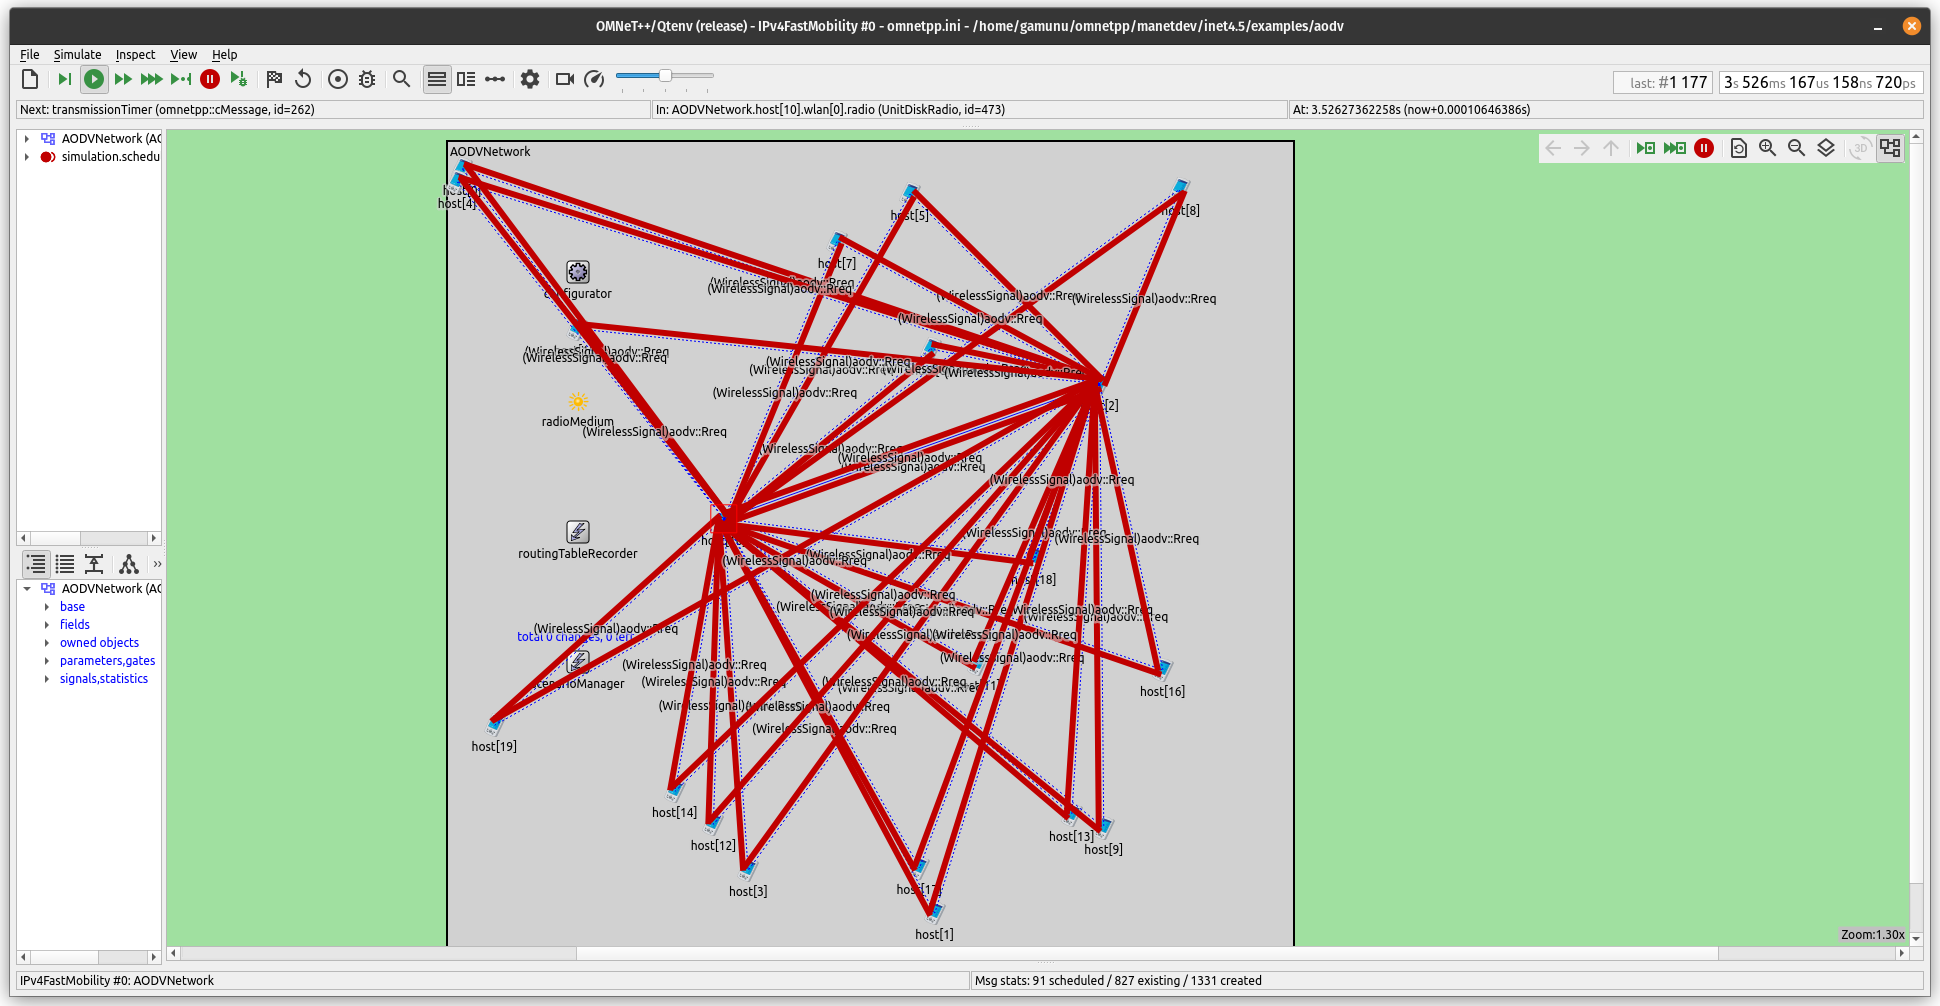
\includegraphics[height=0.45\textwidth]{imgs/aodvSim.png}}
    \caption{AODV protocol network simulation}
    \label{aodvSim}
\end{figure}

\subsubsection{WiFi Direct POC}

To test the feasibility and refine the implementation method, we have developed
a POC application for using WiFi Direct as a communication method. Currently,
communication among clients of the same group is implemented. The group
formation is handled by \texttt{WifiP2pManager}, provided by the Android SDK\cite{wifiman}.